\chapter{微积分}\label{diff-int}
\section{一元微分}
\subsection{导数公式}
\paragraph*{实函数}
\begin{empheq}{align*}
\odv{f(x)}{x}&=f'(x)=\lim_{h\rightarrow 0}\frac{f(x+h)-f(x)}{h}\\
\frac{\dif^n f(ax)}{\dif x^n}&=a^nf^{(n)}(u)\big|_{u=ax}\\
\frac{\dif f(x)}{\dif x}&=\frac{\dif \ln f(x)}{\dif x}f(x)\\
\odv{fg}{x}&=f'g+fg'\\
\odv[order=2]{fg}{x}&=f''g+2f'g'+fg''\\
\odv[order=n]{fg}{x}&=\sum_{k=0}^{n} \binom{n}{k}f^{(k)}g^{(n-k)} 
\end{empheq}

\paragraph*{复函数}
记$z=x+iy,f(z)=u(x,y)+iv(x,y)$,则假如$f$满足柯西——黎曼方程:
\begin{empheq}{align}
\pdv{u}{x}&=\pdv{v}{y}\\
\pdv{u}{y}&=-\pdv{v}{x}
\end{empheq}
那么有复函数的导数:
\begin{empheq}{align}
f'(z)&=\pdv{u}{x}+i\pdv{v}{x}\\
\odv{f(x)e^{ig(x)}}{x}&=f'e^{ig}+fe^{ig}ig'=e^{ig}(f'+ifg')
\end{empheq}

此外常见初等函数$(z^n,\ln z,\sin z,\sinh z,\cdots)$的复导数与实导数形式相同,如$\odv{z^2}{z}=2z$。
\section{多元微分与向量分析}
\subsection{Jacobi矩阵}
多元函数的一阶微分.

\[
J\left(\bm{f}(\bx)\right)=\begin{bmatrix}
\frac{\partial f_1(\bx)}{\partial \bx^T}\\
\cdots\\
\frac{\partial f_n(\bx)}{\partial \bx^T}
\end{bmatrix}
\]

注意我们认为$f$的输出是列向量,它的每一行的导数对应矩阵的1行.
\subsection{向量分析}\label{sec-vector-analysis}
\subsubsection{内积、叉积}

\begin{align*}
\bm{x}\times\bm{y}&=\begin{bmatrix}
\bm{i} &\bm{j}&\bm{k}\\
\bx_1&\bx_2&\bx_3\\
\by_1&\by_2&\by_3
\end{bmatrix} \mtag{叉积}\\
(\bm{x}\bm{y}\bm{z})&=(\bm{x}\times\bm{y})\cdot \bm{z}=\begin{bmatrix}
\bm{x}_1 &\bm{x}_2&\bm{x}_3\\
\by_1&\by_2&\by_3\\
\bz_1&\bz_2&\bz_3
\end{bmatrix} \mtag{混合积}
\end{align*}

显然,混合积满足特殊的交换律:
$$(\bm{x}\bm{y}\bm{z})=(\bm{y}\bm{z}\bm{x})=(\bm{z}\bm{x}\bm{y})=-(\bm{x}\bm{z}\bm{y})=-(\bm{y}\bm{x}\bm{z})=-(\bm{x}\bm{z}\bm{y})$$

叉积还满足的运算规则有:
\begin{align}\label{triple-cross-prod-rule}
\bx\times(\by\times\bz)&=\by(\bx\cdot\bz)-\bz(\bx\cdot\by)
\end{align}
对于三维空间,任取一组基(协变基)$[\bm{e}_1,\bm{e}_2,\bm{e}_3]$,那么对偶基(逆变基)定义为:
$$[\bm{e}^1,\bm{e}^2,\bm{e}^3]=\left[\frac{\bm{e}_2\times\bm{e}_3}{(\bm{e}_1\bm{e}_2\bm{e}_3)},\frac{\bm{e}_3\times\bm{e}_1}{(\bm{e}_1\bm{e}_2\bm{e}_3)},\frac{\bm{e}_1\times\bm{e}_2}{(\bm{e}_1\bm{e}_2\bm{e}_3)}\right]$$

同时对某个向量有分解式
\[
\begin{aligned}
\bm{x}&=x^1\bm{e}_1+x^2\bm{e}_2+x^3\bm{e}_3\\
&=x_1\bm{e}^1+x_2\bm{e}^2+x_3\bm{e}^3
\end{aligned}\]
$[x^1,x^2,x^3]$叫反变坐标,$[x_1,x_2,x_3]$叫共变坐标,这里与张量分析联系起来了。

在笛卡尔坐标系中,共变基与逆变基相同。
\subsubsection{梯度、散度、旋度}
散度是标量场,另两个是向量场。在散度、旋度基本情况下只用来描述3维空间,梯度可以用于任意维度空间。梯度作用于标量场,散度、旋度作用于向量场。

以下假设向量场$\bm{F}=[a(\bm{P}),b(\bm{P}),c(\bm{P})]$,$\bm{P}=[x,y,z]$是三维点。


\paragraph*{哈密顿算子与梯度}用$\nabla$表示哈密顿算子:
$$\nabla =\bm{i}\frac{\partial}{\partial x}+\bm{j}\frac{\partial}{\partial y}+\bm{k}\frac{\partial}{\partial z}$$

标量场的梯度:
$$\textbf{grad } T=\nabla T=[T_x,T_y,T_z]$$
向量场也有梯度,一般就是Jacobi矩阵:$\nabla \bm{F}=J\bm{F}=\pdv{\bm{F^T}}{\bx}=[\bm{F}_x,\bm{F}_y,\bm{F}_z]$,在这样的记号下,$\nabla\cdot(\nabla \bm{F})=\Delta F$,与\eqref{laplacian-of-vector-field}一致。有的地方是用$(J\bm{F})^T$表示$\nabla \bm{F}$,注意区别。

在上面的记号下,
\begin{empheq}{align}
\nabla \cdot(\nabla \bm{F}^T)=\nabla (\nabla\cdot \bm{F})
\end{empheq}

我们还记:
$$(\nabla T)^2=(T_x)^2+(T_y)^2+(T_z)^2$$
不要与$\nabla^2$混淆。

\paragraph*{向量梯度}
$$\frac{\bm{F(P)}}{\partial \bm{n}}=(\bm{n} \textbf{ grad })\bm{F(P)}=(\bm{n}\cdot \nabla)\bm{F}=\lim_{h\rightarrow 0}\frac{\bm{F}(\bm{r}+h\bm{n})-\bm{F(r)}}{h}$$
$\bm{r}$表示向量$\overrightarrow{OP}$,也可以直接用$\bm{P}$表示。一般取$\bm{n}$为单位向量,叫方向导数。注意$\bm{n} \textbf{ grad }$似乎可以理解为向量内积。

对于标量场,方向导数的计算很简单:
\[(\bm{n}\cdot\nabla)f(\bm{x})=\frac{\bm{n}}{|\bm{n}|}\cdot\nabla f(\bm{x})\]

对于向量场有:
\begin{align}
(\bm{n}\cdot\nabla)&=\sum \bm{n}_k\frac{\partial}{\partial x^k}
\end{align}

方向导数在有的地方也表示为
\[\nabla_{\bm{n}}f(\bm{x})\]

\paragraph*{拉普拉斯算子}
\begin{empheq}{align*}
\Delta T(\bm{P})&=\vdiv \textbf{grad } T(\bm{P})\mtag{标量场$\rightarrow$标量}\\
\Delta \bm{F}(\bm{P}) &=\textbf{grad }\vdiv \bm{F(P)}-\textbf{curl }\textbf{curl }\bm{F(P)}\mtag{向量场$\rightarrow$向量}
\end{empheq}
在笛卡尔坐标系下有
\begin{empheq}{align}
\Delta T(\bm{P})&=T_{xx}+T_{yy}+T_{zz}\\
\Delta \bm{F(P)}&=\bm{F}_{xx}+\bm{F}_{yy}+\bm{F}_{zz}\\
\Delta&=\nabla^2=\nabla \cdot \nabla \label{laplacian-of-vector-field}
\end{empheq}

\paragraph*{向量场散度}
$$\vdiv \bm{F}=\nabla \cdot \bm{F}=a_x+b_y+c_z$$

\paragraph*{高阶张量场的散度}前面提到的散度是向量场的散度,结果是标量,对于高阶张量场也可以求散度,一般来说,对$n$阶张量场求散度后得到$n-1$阶张量。比如流体力学中的
\begin{empheq}{align}
\vdiv (\bm{U}\bm{U})&\coloneqq \vdiv (\bm{U}\otimes \bm{U})\\
&=\vdiv \begin{bmatrix}
u_1u_1& u_1u_2& u_1u_3\\
u_2u_1& u_2u_2& u_2u_3\\
u_3u_1& u_3u_2& u_3u_3
\end{bmatrix}\\
&=\begin{bmatrix}
\vdiv [u_1u_1,u_1u_2,u_1u_3]\\
\vdiv [u_2u_1,u_2u_2,u_2u_3]\\
\vdiv [u_3u_1,u_3u_2,u_3u_3]
\end{bmatrix}\\
&=(\nabla \bm{U})\bm{U}+(\vdiv \bm{U})\bm{U}\\
&=\bm{U}\cdot \nabla \bm{U}+\bm{U}\nabla \cdot \bm{U}
\end{empheq}
\paragraph*{向量场旋度}
$$\textbf{curl\ } \bm{F}=\nabla\times \bm{F}=[c_y-b_z,a_z-c_x,b_x-a_y]=\begin{bmatrix}
\bm{i} & \bm{j} &\bm{k}\\
\frac{\partial}{\partial x} & \frac{\partial}{\partial x}& \frac{\partial}{\partial x}\\
a& b& c
\end{bmatrix}$$

在爱因斯坦符号下,给定向量场$\bm{F}=\left[F_1,F_2,F_3\right]$,有
\[\nabla\times\bm{F}=\varepsilon^{ijk}\bm{e}_i\frac{\partial F_k}{\partial x^j}\]

\paragraph*{运算法则}由于梯度、散度、旋度都是线性算子,所以线性算子的运算性质就不列出了。

涉及梯度的:

\begin{empheq}{align}
\nabla (ab)&=(\nabla a)b+a(\nabla b)\\
\nabla (\varphi \bm{a})&=(\nabla \varphi)\cdot \bm{a}+\varphi \vdiv \bm{a}\\
\nabla (\bm{a}\cdot \bm{b})&=\bm{a}\times(\nabla \times \bm{b})+\bm{b}\times(\nabla\times \bm{a}) + (\bm{a}\cdot\nabla )\bm{b}+(\bm{b}\cdot \nabla )\bm{a}\label{div-of-inner-prod}\\
\vdiv (\rho \bm{F}\bm{F})&=(\nabla \rho \bm{F})F+(\vdiv \rho\bm{F})\bm{F}
\end{empheq}

涉及散度的:
\[
\begin{aligned}
\vdiv (\bm{a}\times \bm{b})&=(\nabla\times \bm{a})\cdot\bm{b}-\bm{a}\cdot(\nabla\times\bm{b})\\
\vdiv \vcurl \bm{a}&=\nabla\cdot(\nabla\times \bm{a})=0
\end{aligned}
\]

涉及拉普拉斯算子的:
\begin{empheq}{align}
\Delta(ab)&=(\Delta a)b+2\nabla a\cdot\nabla b+a(\Delta b)\\
\Delta f(g(\bx))&=f''(g)(\nabla g)^2+f'(g)\Delta g\\
\Delta (ae^{g})&=e^g\left(\Delta a+2\nabla a\cdot \nabla g+a((\nabla g)^2+\Delta g)\right)\\
\Delta (\bm{a}\cdot \bm{b})&=()
\end{empheq}


涉及旋度的:
\begin{empheq}{align}
\nabla \times \pdv{\bm{F}}{t}&=\pdv{}{t}(\nabla \times \bm{F})\\
\nabla\times(\nabla \phi)&=0\\
\nabla^2\phi&=\nabla\cdot(\nabla \phi)\\
\nabla\times(\nabla\times \bm{a})&=\nabla(\nabla\cdot \bm{a})-\nabla^2\bm{a}\\
\nabla \times (f\bm{F})&=f(\nabla\times \bm{F})+(\nabla f)\times\bm{F}\\
\nabla\times(\bm{a}\times\bm{b})&=\bm{a}(\nabla\times \bm{b})-\bm{b}(\nabla\cdot\bm{a})+(\bm{b}\cdot\nabla)\bm{a}-(\bm{a}\cdot\nabla)\bm{b}\\
&=(\nabla\cdot \bm{b}+\bm{b}\cdot\nabla)\bm{a}-(\nabla\cdot\bm{a}+\bm{a}\cdot\nabla)\bm{b}\\
&=\nabla\cdot(\bm{b}\bm{a}^T)-\nabla\cdot(\bm{a}\bm{b}^T)\\
&=\nabla\cdot(\bm{b}\bm{a}^T-\bm{a}\bm{b}^T)
\end{empheq}

涉及三维位矢$\bm{r}=[x,y,z]$的:
\begin{empheq}{align}
\nabla \bm{r}&=\frac{\bm{r}}{r}\\
\nabla \phi(r)&=\phi'(r)\frac{\bm{r}}{r}\\
\nabla \frac{1}{r}&=-\frac{\bm{r}}{r}\\
\nabla (\bm{c}\cdot \bm{r})&=(\bm{c}\cdot\nabla)\bm{r}=\bm{c}\\
\nabla e^{i(\bm{c}\cdot\bm{r})}&=ie^{i(\bm{c}\cdot\bm{r})}\bm{c}\\
\nabla^2 \inv{r}&=-\nabla\cdot\left(\frac{\bm{r}}{r^3}\right)
\end{empheq}

\begin{empheq}{align}
\nabla\cdot\bm{r}&=3
\end{empheq}

\begin{empheq}{align}
\nabla\times\bm{r}&=\bm{0}\\
\end{empheq}

以上记$r=|\bm{r}|$,$\bm{c}$为常矢量。
\subsubsection{向量分析基本定理}
\paragraph*{无散场}\label{vec-ana-div-zero}如果向量场$\bm{f}$的散度为$0$,则它叫作无散场或横场、无源场。同时有
$$\vdiv \bm{f}=0\implies \exists \bm{A},\bm{f}=\nabla\times \bm{A}$$
无源场这个名字更能反映散度的本质,如果散度为0,就表示不存在源,不能“无中生有”。
\paragraph*{无旋场}旋度为0的向量场叫无旋场或者纵场。有:
$$\vcurl=0\implies \exists \phi,\bm{f}=\nabla \phi$$
此处$\phi$为标量场。
\paragraph*{向量场的唯一性}一个向量场$\bm{f}$由散度、旋度、边界条件唯一确定。
\paragraph*{亥姆霍兹定理}矢量场的分解定理:
\begin{theorem}[亥姆霍兹定理]
任意一个向量场可以分解为无旋场与无散场之和:
$$\bm{f}=\bm{f}_1+\bm{f}_2=\nabla \phi+\nabla \times \bm{A}$$
\end{theorem}


\subsection{复函数的向量分析}
\subsubsection{梯度、散度、旋度}

\paragraph*{运算法则}运算法则与实数的相似。

涉及梯度的:
\begin{empheq}{align}
\nabla e^{iS(x,y,z)}&=ie^{iS}\nabla S\\
\nabla a(x,y,z)e^{iS(x,y,z)}&=(\nabla a)e^{iS}+iae^{iS}(\nabla S)
\end{empheq}

涉及拉普拉斯算子的:
\begin{empheq}{align}
\Delta e^{iS(x,y,z)}&=e^{iS}(i\nabla S)^2+ie^{iS}\Delta S=-e^{iS}(\nabla S)^2+ie^{iS}\Delta S\\
\Delta a(x,y,z)e^{iS(x,y,z)}&=e^{iS}\left(\Delta a+2i\nabla a\cdot\nabla S+a\left(-(\nabla S)^2+i\Delta S\right)\right)
\end{empheq}

\section{差分逼近}\label{diff-int-finite-difference}
\subsection{一维}
\subsubsection{一致网格}
这里的一致是指网格的大小相同。最基本的几个差分公式:
\begin{empheq}{align*}
f'(x)&=\frac{f(x+h)-f(x)}{h}\\
&=\frac{f(x+h)-f(x-h)}{2h}(\text{精度更高})\\
\end{empheq}

可以按如下方式推导差分逼近的公式。考虑“五点式”逼近一阶导数,由Taylor公式可以给出
\begin{empheq}{equation}
\begin{bmatrix}
f(x+2h)\\
f(x+h)\\
f(x)\\
f(x-h)\\
f(x-2h)
\end{bmatrix}=\begin{bmatrix}
1 & 2h & \frac{(2h)^2}{2} & \frac{(2h)^3}{3!} & \frac{(2h)^4}{4!}\\
1 & h & \frac{h^2}{2} & \frac{h^3}{3!} &  \frac{h^4}{4!}\\
1 &0 & 0& 0& 0\\
1 & -h & \frac{h^2}{2} & -\frac{h^3}{3!} &  \frac{h^4}{4!}\\
1 & -2h & \frac{(2h)^2}{2} & -\frac{(2h)^3}{3!} & \frac{(2h)^4}{4!}
\end{bmatrix}\begin{bmatrix}
f(x)\\
f'(x)\\
f''(x)\\
f'''(x)\\
f^{(4)}(x)
\end{bmatrix}
\end{empheq}
对应于
$$F=AF'$$

现在我们希望求$F$的线性组合,使得
$$c^TF=C^TAF'=\begin{bmatrix}
0 & 1 & 0 & 0 & 0
\end{bmatrix}F'=f'(x)$$

那么
$$c^T=\begin{bmatrix}
0 & 1 & 0 & 0 & 0
\end{bmatrix}A^{-1}$$

可以看出,通过使用更多的点,可以消去高阶导数。以上的方程组还可以用来推导2、3、4阶导数的近似公式。

类似地可以考虑一阶导数的前向差分,
$$A=\begin{bmatrix}
1 & h\\1&0
\end{bmatrix}$$
则逼近方式为
$$f'(x)=c^TF=\begin{bmatrix}
0 & 1 
\end{bmatrix}\begin{bmatrix}
1 & h\\1&0
\end{bmatrix}^{-1}F=\begin{bmatrix}
0 & 1 
\end{bmatrix}\begin{bmatrix}
0 & 1\\\frac{1}{h}&-\frac{1}{h}
\end{bmatrix}F=\begin{bmatrix}
\inv{h} & -\inv{h} 
\end{bmatrix}\begin{bmatrix}
f(x+h)\\f(x)
\end{bmatrix}$$

对于一阶导数的中心差分:
$$A=\begin{bmatrix}
1 & h & \frac{h^2}{2}\\
1 & 0 & 0\\
1 & -h & \frac{h^2}{2}
\end{bmatrix}$$
那么
$$f'(x)=\begin{bmatrix}
0 & 1 & 0
\end{bmatrix}A^{-1}F=\begin{bmatrix}
\inv{2h} & 0 & -\inv{2h} 
\end{bmatrix}\begin{bmatrix}
f(x+h)\\f(x)\\f(x-h)
\end{bmatrix}$$
\subsubsection{非一致网格}
\paragraph*{Hilding Sundqvist}文献\cite{https://doi.org/10.1111/j.2153-3490.1970.tb01933.x}提出了一种非均匀网格的离散方法:
\begin{empheq}{align}
f_i'&=\frac{f_{i+1}-\left(\frac{h_k}{h_{k-1}}\right)^2f_{i-1}-\left(1-\left(\frac{h_k}{h_{k-1}}\right)^2\right)f_i}{h_k\left(1+\frac{h_k}{h_{k-1}}\right)}+\mathcal{O}(h_kh_{k-1}f_i''')\\
f_i''&=2\frac{f_{i+1}+\left(\frac{h_k}{h_{k-1}}\right)f_{i-1}-\left(1+\frac{h_k}{h_{k-1}}\right)f_i}{h_kh_{k-1}\left(1+\frac{h_k}{h_{k-1}}\right)}+\mathcal{O}((h_k-h_{k-1})f_i''')
\end{empheq}

图示如下:
\begin{center}
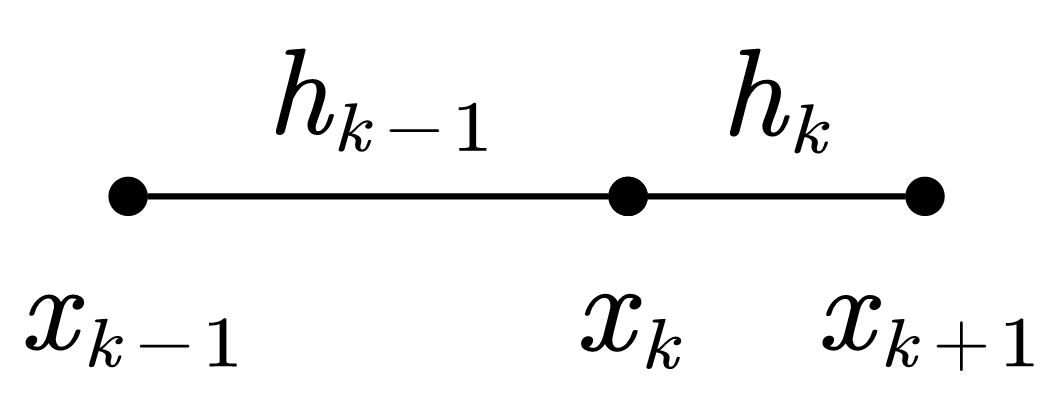
\includegraphics[width=3cm]{figure/Hingding-nonuniform-grid.png}
\end{center}

\subsection{二维}
\subsubsection{一致网格}
\paragraph*{梯度与Hessian阵}
\begin{empheq}{align}
\left.\pdv[order=2]{f}{x}\right|_{i,j}&=\frac{f_{i+1,j}-2f_{i,j}+f_{i-1,j}}{h^2}+\mathcal{O}(h^2)\\
\left.\pdv[order=2]{f}{y}\right|_{i,j}&=\frac{f_{i,j+1}-2f_{i,j}+f_{i,j-1}}{k^2}+\mathcal{O}(k^2)\\
\left.\pdv[order={1,1}]{f}{x,y}\right|_{i,j}&=\frac{f_{i+1,j+1}-f_{i+1,j-1}-f_{i-1,j+1}+f_{i-1,j-1}}{4hk}\mtag{四对角}\\
&=\frac{f_{i+1,j+1}-f_{i+1,j}-f_{i,j+1}+2f_{i,j}-f_{i-1,j}-f_{i,j-1}+f_{i-1,j-1}}{2hk}\mtag{七对角}
\end{empheq}
以上$f_{i+1,j+1}=f(x+h,y+k)$,其它类似。

注意在$f_{xy}$的第二个公式中,假如我们是依次计算$f_x,f_y,f_{xx},f_{yy}$,那么只需要再计算$f(x+h,y+k),f(x-h,y-k)$就可以计算$f_{xy}$了,$f(x+h,y)$一类可以利用之前计算的值。前两个$f_{xx},f_{yy}$实际上是固定另一个变量,然后进行一维差分。

图示如下:
\begin{center}
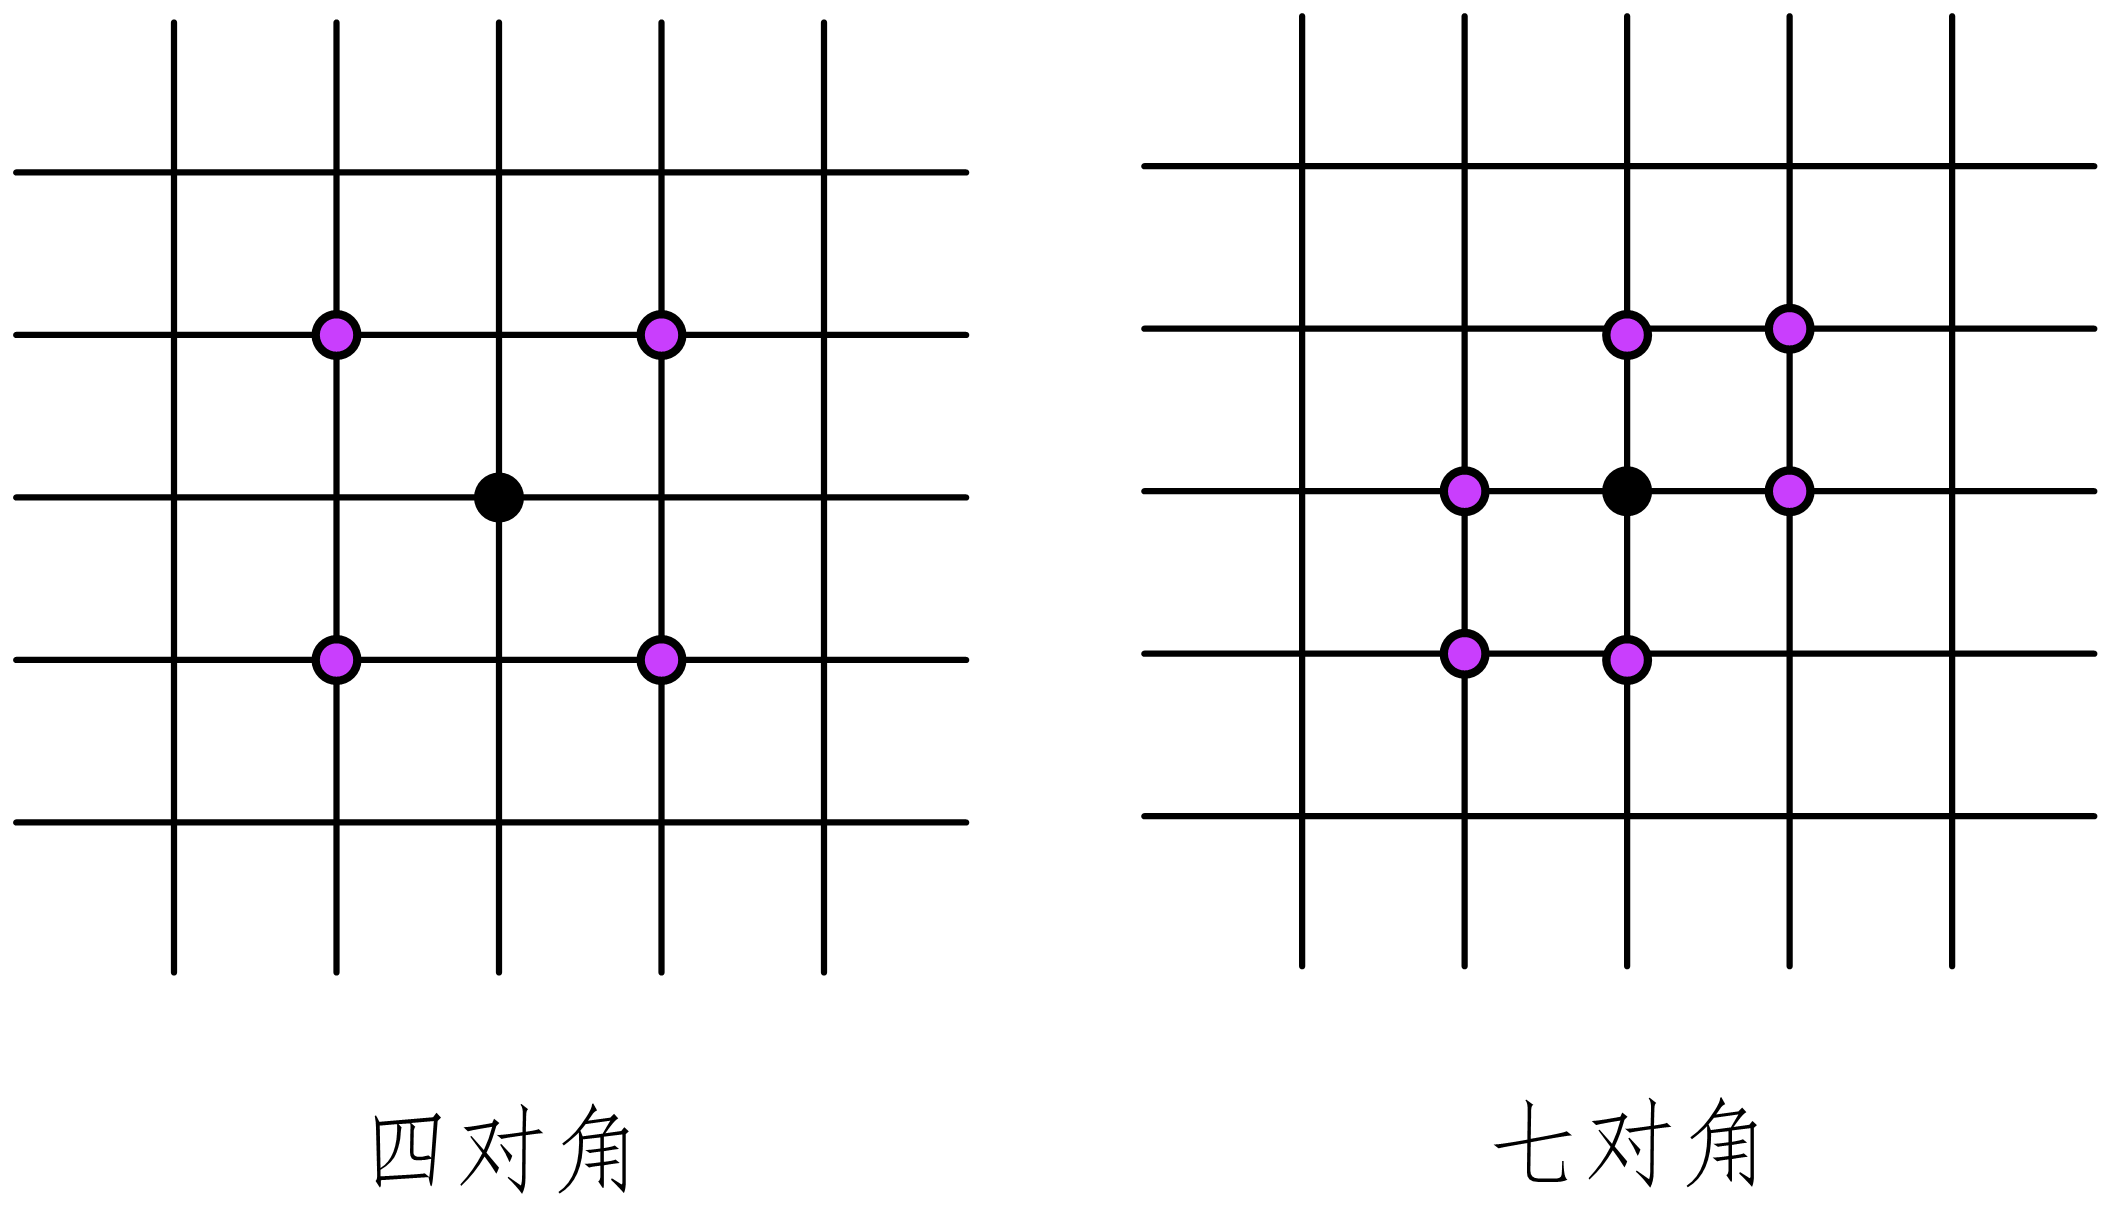
\includegraphics[width=10cm]{figure/2D-uniform-finite-difference.png}
\end{center}

\paragraph*{Laplacian}
\begin{empheq}{align}
\nabla^2 f|_{i,j}&=\left.\pdv[order=2]{f}{x}\right|_{i,j}+\left.\pdv[order=2]{f}{x}\right|_{i,j}-\inv{12}hk(f_{xxxx}+f_{yyyy})+\mathcal{O}(h^2k^2)\mtag{五点式}\\
&=\inv{6hk}(4f_{i-1,j}+4f_{i+1,j}+4f_{i,j-1}+4f_{i,j+1}\mtag{九点式}\\
&\qquad +f_{i-1,j-1}+f_{i-1,j+1}+f_{i+1,j-1}+f_{i+1,j+1}-20f_{i,j})\nonumber\\
&\qquad -\inv{12}hk(f_{xxxx}+2f_{xxyy}+f_{yyyy})+\mathcal{O}(h^2k^2)\nonumber
\end{empheq}
这里的五点式是指二阶导数用前面的中心差分。九点式已经把周围的点全用上了。

在9点式中,注意
\begin{empheq}{align}
f_{xxxx}+2f_{xxyy}+f_{yyyy}=\nabla^2(\nabla^2f)
\end{empheq}
所以可以在不求得解的情况下计算主误差。

\subsubsection{非一致网格}

\subsection{三维}
\subsubsection{一致网格}

\subsubsection{非一致网格}

\section{特殊微分与导数}
\subsection{Frechet导数}
\subsubsection{定义}

\subsection{Gateaux导数}

\subsection{Dini导数}

\section{微分算子}
\subsection{流与向量场}
\subsubsection{向量场}\label{vector-field}
\begin{definition}[向量场]
一个向量场是一个光滑映射:
$$X:U\rightarrow \Rns$$
其中$U\subset \Rns$是一个开集。

考虑一个对应的ODE:
$$\by'=X(\by),\by(0)=\bx$$
它的解$\by(t):\mathbb{R}\rightarrow\Rns$被称为向量场的积分曲线,或者轨道。同时记解
$$\by=\by(t,\bx)=\mathcal{F}_X^t(\bx)$$
这里的$\bx$是初值,是定值。$\mathcal{F}_X^t$被称为向量场产生的流,所以流是向量场的积分。

向量场定义了一个标量函数的微分算子:
$$\mathcal{L}_Xf(\bx)=\lim_{h\rightarrow 0}\frac{f(\mathcal{F}_X^t\bx)-f(\bx)}{h}=\left.\odv{}{t}f(\mathcal{F}_X^t\bx)\right|_{t=0}$$
也记为$\mathcal{L}_X f(\bx)=Xf$。根据微分法则有:
$$\mathcal{L}_X f(\bx)=X(\bx)\cdot \nabla f(\bx)=\sum a_j(\bx)\pdv{f}{x_j}$$
\end{definition}
把向量场作为速度场,在空间中选择一个起点$\bx$,在速度场的作用下进行运动,在空间中画出一条轨迹,就是流。

$\mathcal{L}_X f(\bx)$可以理解为:在微小的时间内,在速度场的作用下从一个点运动到另一个点,由此引起了标量函数的变化,从而可以定义导数。

\subsubsection{李导数}
\begin{definition}[李导数]

\end{definition}
\subsection{微分形式}
\subsubsection{$k$形式}
\begin{definition}[1-形式]
一个$\Omega\in\Rns$上的1-形式表示为
$$\alpha=\sum_j a_j(\bx)\dif x_j$$
假如$\gamma:[a,b]\rightarrow \Omega$是一条光滑曲线,则有
$$\int_{\gamma} \alpha=\int_a^b \sum_j a_j(\gamma(t))\gamma_j'(t)\dif t=\int_I \gamma^{\ast}\alpha$$
$\gamma^{\ast}$是$\alpha$在映射$\gamma$下的拉回。
\end{definition}

\begin{definition}[$k$-形式]
一个$\Omega$上的$k$-形式$\alpha$是一个向量场上的$k$重多线性映射:
$$\alpha(X_1,\cdots,X_k)\in C^{\infty}(\Omega)$$
它满足反对称性:
$$\alpha(X_,\cdots,X_j,\cdots,X_l,\cdots,X_k)=-\alpha(X_,\cdots,X_l,\cdots,X_j,\cdots,X_k)$$

$k$-形式记为
\begin{empheq}{equation}\label{diff-k-form}
\alpha=\sum_j a_j(\bx)\dif x_{j_1}\wedge\cdots\wedge \dif x_{j_k}
\end{empheq}
其中
$$a_j(\bx)=\alpha(D_{j_1},\cdots,D_{j_k}),\quad D_j=\pdv{}{x_j}$$
求和是对所有$k$-元组$(j_1,\cdots,j_k)$进行的,同时有:
$$\dif x_{j_1}\wedge \cdots \wedge \dif x_{j_k}=(\sgn \sigma)\dif x_{j_{\sigma(1)}}\wedge \cdots\wedge\dif x_{j_{\sigma(k)}}$$
$\sigma$是$\{1,\cdots,k\}$的一个排列。如果$j_m=j_l$,则上式为0。

一个$k$-形式也记为
$$\alpha\in\Lambda^{k}(\Omega)$$
\end{definition}

\subsubsection{微分形式的运算}
\paragraph*{外积}相当于微分形式的“乘法”。
\begin{definition}[外积wedgep product] 
假如$\alpha\in\Lambda^k(\Omega)$由\ref{diff-k-form}给出,而
$$\beta=\sum_i b_i(\bx)\dif x_{j_1}\wedge\cdots\wedge\dif x_{i_l}\in\Lambda^l(\Omega)$$
则有外积
$$\alpha\wedge\beta=\sum_{j,i}a_j(\bx)b_i(\bx)\dif x_{j_1}\wedge\cdots\wedge\dif x_{j_k}\wedge\dif x_{i_1}\wedge\cdots\wedge\dif x_{i_l}=(-1)^{kl}\beta\wedge\alpha$$
对于一些特殊情形有以下记号:
$$\wedge_k \alpha=\dif x_k\wedge\alpha$$
\end{definition}
上面$a_jb_i$的形式有点类似于向量的外积$\bx\by^T$,而$\dif$项是直接拼在一起的。

\paragraph*{内积}此“内积”(interior product)不是Hilbert空间中的内积。
\begin{definition}[内积interior product]
也叫contraction。定义为
$$(\alpha\rfloor X)(X_1,\cdots,X_{k-1})=\alpha(X,X_1,\cdots,X_{k-1})\in\Lambda^{k-1}(\Omega)$$
也可以记为$i_X\alpha$。

特殊记号:
$i_k\alpha=\alpha \rfloor D_k$。
\end{definition}
contraction可能比interior product更加形象。有点类似于消去一个参数。在Matlab中定义function handle的时候有类似的操作:
\begin{center}
\texttt{new\_fun=@(y) fun(x,y)}
\end{center}


\paragraph*{外微分}对微分形式进行微分。
\begin{definition}[外微分exterior derivative]
外微分$d:\Lambda^k(\Omega)\rightarrow\Lambda^{k+1}(\Omega)$定义为:
$$\dif \alpha=\sum_{j,l}\pdv{a_j}{x_l}\dif x_l\wedge x_{j_1}\wedge\cdots\wedge \dif x_{j_k}$$

它满足性质
\begin{enumerate}
\item $\dif(\dif \alpha)=0$。
\item $\dif(\alpha\wedge\beta)=(\dif \alpha)\wedge \beta+(-1)^k\alpha\wedge(\dif\beta),\quad\alpha\in\Lambda^k(\Omega),\beta\in\Lambda^j(\Omega)$
\item $F^{\ast}(\dif\alpha)=\dif (F^{\ast}\alpha)$
\end{enumerate}
\end{definition}

外微分有一个著名的定理:
\begin{theorem}[外微分定理]
\begin{empheq}{equation}
\int_{\Omega}\dif \alpha=\int_{\partial \Omega} \omega
\end{empheq}
\end{theorem}
它把全区域的积分转换成了边界上的积分,牛顿-莱布尼茨公式、格林公式、高斯公式都是它的特例。
\paragraph*{关系}
\begin{empheq}{align}
\wedge_k \iota_l+\iota_l\wedge_k&=\delta_{kl}\mtag{反交换}\\
\wedge_j\wedge_k+\wedge_k\wedge_l&=0\\
\iota_j\iota_k+\iota_k\iota_j&=0
\end{empheq}

\subsection{Halmiltonian系统}


\section{一元积分}
注意有的文章里面没有使用标准符号,比如\cite{10.2307.3215821}中,
$$\int_{0}^{\infty}\dif h\ G(h)$$
其实是表示 
$$\int_{0}^{\infty}G(h)\dif h$$
而不是
$$\int_{0}^{\infty}\dif (hG(h))$$
\subsection{定积分}
\subsubsection{微积分基本公式}
\begin{empheq}{equation}
\int_{a}^{b}\dif F(x)=F(b)-F(a)
\end{empheq}
\section{曲线积分}
\subsection{对线元曲线积分}
对线元的积分:
\begin{empheq}{equation}
\int_L f(\bx)\dif s
\end{empheq}
$L$是一段曲线,$\dif s$为线元。

在曲线自然参数化下,曲线表示为弧长的函数:$L=\bx(s)$,此时原积分为
$$\int_{s_0}^{s_1} f(\bx(s))\dif s$$

假如曲线可以由参数曲线$L=\bx(t)$,则$\dif s=\sqrt{\sum \left(\odv{x_k}{t}\right)^2}$,则原积分为:
$$\int_{t_0}^{t_1} f(\bx(t))\sqrt{\sum \left(\odv{x_k}{t}\right)^2}\dif t$$

假如曲线可以转化为某个坐标$x_i$的函数则原积分为:
$$\int_{x_0}^{x_1} f(\bx(x_i))\sqrt{\sum \left(\odv{x_k}{x_i}\right)^2}\dif x_i$$
跟$t$参数化是一回事。

假如曲线可以由一个单参数化经过坐标变换给出:$L=\bx(\by(t)))$。则$\dif \bx=J\by'\dif t$,$\dif s=\sqrt{(\dif \bx)^T(\dif \bx)}=\sqrt{(\by')^TJ^TJ\by'}\dif t=\sqrt{g_{ij}\dif y^i\dif y^j}$。参考\ref{tensor-field-metric}。

比如对于极坐标系,$t=\theta,\by=(r,\theta),\by'=(r',1)$,有
$$\int_L f(x,y)\dif s=\int_{\theta_0}^{\theta_1}f(r(\theta)\cos\theta,r(\theta)\sin\theta)\sqrt{r^2(\theta)+(r'(\theta))^2}\dif \theta$$
\subsection{对坐标曲线积分}
对坐标的积分:
$$\int_L \sum a_k(\bx)\dif x_k$$
这个一般可以每一项分开算,把曲线$L$分别转换成$x_k$的函数,然后再当成一元积分。

也可以常规换元:
$$\int_{t_0}^{t_1}\sum a_k(\bx(t))x_k'\dif t$$

\subsection{联系与区别}
\begin{enumerate}
\item 第一类曲线积分与第二类曲线积分可以相互转化:
$$\int_L \sum a_k(\bx)\dif x_k=\int_L \sum a_k(\bx)\cos\theta_k\dif s$$
$\theta_k$为有向曲线弧的单位切向量。实际上给定一个向量$\dif s$,则它在某方向的投影长就是$(\dif s)\theta_k=\dif x_k$,所以上式也相当于换元。
\end{enumerate}
\subsection{例题}

\section{重积分}
\subsection{二重积分}
\subsubsection{一般二重积分}
\paragraph*{一般形式}笛卡尔坐标系下:
\begin{empheq}{equation}
\int_{\Omega}f(x,y)\dif x\dif y=\int_{x_0}^{x_1}\int_{y_0(x)}^{y_1(x)}f(x,y)\dif y\dif x
\end{empheq}

极坐标系下:
\begin{empheq}{equation}
\int_{\Omega}f(r,\theta)r\dif r\dif \theta=\int_{\theta_0}^{\theta_1}\int_{r_0(\theta)}^{yr_1(\theta)}f(r,\theta)r\dif r\dif \theta
\end{empheq}

\subsubsection{对面积曲面积分}
\paragraph*{基本形式}
\begin{empheq}{equation}
\int_{\Sigma} f(x,y,z)\dif S
\end{empheq}
这里的$\dif S$是曲面上一个小的面积元,注意它不是$\dif x\dif y$。 
\paragraph*{投影法}假如$\Sigma$可以投影到某个坐标面上,比如$xOy$,则有
\begin{empheq}{equation}\label{2d-int-area-project}
\int_{\Sigma} f(x,y,z)\dif S=\int_{D_{xy}}f(x,y,z(x,y))\sqrt{1+z_x^2+z_y^2}\dif x\dif y
\end{empheq}

\subsubsection{对坐标曲面积分}
\paragraph*{基本形式}
\begin{empheq}{equation}
\int_{\Sigma} f(x,y,z)\dif x\dif y
\end{empheq}
\paragraph*{投影法}假如$\Sigma$可以投影到某个坐标面上,比如$xOy$,则有
\begin{empheq}{equation}
\int_{\Sigma} f(x,y,z)\dif x\dif y=\pm\int_{D_{xy}}f(x,y,z(x,y))\dif x\dif y
\end{empheq}
注意与面积的曲面积分式\cref{2d-int-area-project}不同,被积表达式没有根号那一项。而且符号有正负。一般外法向定义为正。 

\subsubsection{两类曲面积分的联系}
\paragraph*{基本原理}
\begin{empheq}{equation}
\int_{\Sigma} P\dif y\dif z+Q\dif x\dif z+R\dif x\dif y=\int_{\Sigma} P\cos\alpha+Q\cos\beta+R\cos\gamma\dif S
\end{empheq}

\subsubsection{格林公式}\label{green-formula}
\paragraph*{基本原理}把二维封闭曲面积分转换成边界上的二维曲线积分:
\begin{empheq}{equation}
\int_{\Omega}\left(\pdv{Q}{x}-\pdv{P}{y}\right)\dif x\dif y=\int_{L^+}  P\dif x+Q\dif y
\end{empheq}
这里的$L^+$表示正向,沿着曲线走,曲面总在左边的方向为正,直观就是逆时针。

\paragraph*{有限元基本公式}以下假定$\Omega$为一平面区域。这个积分出现在拉普拉斯方程的有限元法中:
\begin{empheq}{align}
\langle -\Delta u, v\rangle&=\iint_{\Omega} v\Delta u\dif x\dif y\\
&=-\iint_{\Omega} \left(\underbrace{((u_xv)_x+(u_y v)_y)}_{\text{格式公式}}-u_xv_x-u_yv_y\right)\dif x\dif y\\
&=-\int_{\partial \Omega} u_x v\dif y-u_y v\dif x+\iint_{\Omega} u_xv_x+u_yv_y\dif x\dif y
\end{empheq}

假如$u,v$在边界$\partial \Omega$上为0,则原式变成:
\begin{empheq}{equation}
\langle -\Delta u, v\rangle=\iint_{\Omega} u_xv_x+u_yv_y\dif x\dif y
\end{empheq}

\subsubsection{斯托克斯公式}\label{2d-surface-int-stokes-theorem}
\paragraph*{基本原理}把三维封闭曲面积分转换成边界上的三维曲线积分:
\begin{empheq}{align}
&\int_{\Sigma}\left(\pdv{R}{y}-\pdv{Q}{z}\right)\dif y\dif z+\left(\pdv{P}{z}-\pdv{R}{x}\right)\dif x\dif z+\left(\pdv{Q}{x}-\pdv{P}{y}\right)\dif x\dif y\\
=&\int_{\Sigma}\begin{vmatrix}
\dif y \dif z& \dif z\dif x & \dif x\dif y \\
P & Q& R\\
\pdv{}{x}& \pdv{}{y}&\pdv{}{z}
\end{vmatrix}\\
=&\int_{L^+} P\dif x+Q\dif y+R\dif z
\end{empheq}
这里的正向符合右手法则:除大拇指外手指绕曲线时,大拇指指的方向为正向。

\subsubsection{曲面面积}
\paragraph*{面积的计算}熟知一个平面曲面$D$的面积在笛卡尔系下表示为:
\begin{empheq}{align}
S=\iint_{D}\dif x\dif y=\int_{x_0}^{x_1}\int_{y_0(x)}^{y_1(x)}\dif y\dif x
\end{empheq}

在极坐标系下为:
\begin{empheq}{align}
S=\iint_{D}r\dif r\dif \theta=\int_{\theta_0}^{\theta_1}\int_{r_0(\theta)}^{r_1(\theta)}r\dif r\dif \theta
\end{empheq}
但使用极坐标计算务必需要$\Sigma$包含原点,且为简单曲面。否则会出错。

如果使用斯托克斯公式\ref{2d-surface-int-stokes-theorem},则面积可以改写为:
\begin{empheq}{align}
S&=\iint_{D}\dif x\dif y\\
&=-\oint_{L^+}y\dif x\\
&=\oint_{L^+} x\dif y\\
&=\inv{2}\oint_{L^+} x\dif y-y\dif x
\end{empheq}
这样就转换成了一个曲线积分的问题,假如曲面是由参数方程给出的,则计算较为方便。但务必注意曲线不能自交。

\paragraph*{参数曲面算例}
\begin{example}
考虑一个参数曲面:$x=\cos 2t,y=t\sin t,0\leq t\leq 2\pi$所围图形的面积。

该参数曲线如下图所示:
\begin{center}
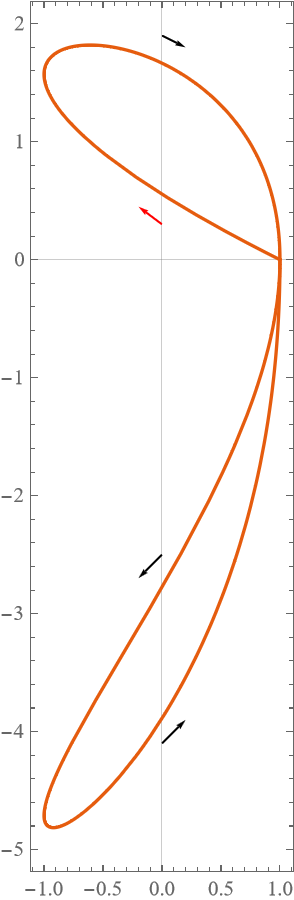
\includegraphics[width=4cm]{figure/two-curve.png}
\end{center}
红色箭头为起始方向。
\end{example}
\begin{solution}
由于曲线是自交的,所以需要分两段计算。
\begin{empheq}{align*}
S&=-\left(-\int_{0}^{\pi} y\dif x\right)-\int_{\pi}^{2\pi}y\dif x\\
&=-2\int_{0}^{\pi}t\sin t \sin (2t)\dif t +2\int_{\pi}^{2\pi}t\sin t \sin (2t)\dif t\\
&=\frac{16}{9}+\frac{16}{9}\\
&=\frac{32}{9}
\end{empheq}
第一项的前面有个负号,是因为沿图中红色箭头方向出发时,曲面在右边,但曲面在左边时才定义为正,所以需要取反。
\end{solution}
\subsection{三重积分}
\subsubsection{一般三重积分}
\paragraph*{基本形式}
\begin{empheq}{equation}
\int_{\Omega}f(x,y,z)\dif V=\int_{x_0}^{x_1}\int_{y_0(x)}^{y_1(x)}\int_{z_0(x,y)}^{z_1(x,y)}f(x,y,z)\dif z\dif y\dif x
\end{empheq}
上式中$\dif V=\dif x\dif y\dif  z$,物理学中有时也记为$\dif^3 x$。

\paragraph*{球坐标}

\subsubsection{高斯公式}
\paragraph*{基本原理}高斯公式建立了体积分与曲面积分的联系,把体积分变成边界上的对坐标曲面积分。 
\begin{empheq}{equation}
\int_{\Omega}\left(\pdv{P}{x}+\pdv{Q}{y}+\pdv{R}{z}\right)\dif x\dif y\dif z=\int_{\partial\Omega}  P\dif y\dif z+Q\dif x\dif z+R\dif x\dif y
\end{empheq}

\paragraph*{泊松方程3D有限元基本公式}以下$\Omega$为一3D区域。积分出现在3D泊松方程的有限元法中,利用高斯公式可以证明:
\begin{empheq}{align}
\langle -\Delta u,v\rangle &=-\iiint_{\Omega} v\Delta u\dif V\\
&=-\iiint_{\Omega} (u_xv)_x+(u_yv)_y+(u_zv)_z-(u_xv_x+u_yv_y+u_zv_z)\dif V\\
&=-\iint_{\partial \Omega} u_xv\dif y\dif z +u_yv\dif x\dif z+u_zv\dif x\dif y+\iiint_{\Omega}\nabla u\cdot\nabla v\dif V
\end{empheq}

假如在边界上$v$为0,则
\begin{empheq}{equation}
\langle -\Delta u,v\rangle =\iiint_{\Omega}\nabla u\cdot\nabla v\dif V
\end{empheq}


\subsubsection{旋转体}

\section{数值积分}
\subsection{插值型求积}
\subsubsection{简介}

\subsubsection{牛顿-柯茨法}

\subsubsection{高斯求积}

\subsection{复化求积}
\subsubsection{基本原理}
对于一维函数,把区间$[a,b]$分隔为多个小区间得到节点$[x_0,\cdots,x_n]$,在每个小区间上进行近似:
\begin{empheq}{equation}
I=\int_{a}^{b} f(x)\dif x=\sum_{k=0}^{n-1} \int_{x_k}^{x_{k+1}} f(x)\dif x
\end{empheq}
小区域积分$\int_{x_k}^{x_{k+1}} f(x)\dif x$可以用前面的插值型积分来计算。
\subsubsection{梯形法则}
用梯形来逼近积分:
\begin{empheq}{equation}
\int_{x_k}^{x_{k+1}} f(x)\dif x=\frac{(f(x_k)+f(x_{k+1}))(x_{k+1}-x_k)}{2}
\end{empheq}

\section{积分表}
\subsection{基本函数}

\subsection{三角函数}
\begin{align}
\int_{-\infty}^{\infty} \frac{\sin^2 x}{x^2}\dif x&=\pi
\end{align}

\subsection{超越函数}

\subsection{有理函数}

\subsection{无理函数}
\begin{empheq}{align}
\int \frac{\dif x}{\sqrt{ax^2+bx+c}}&=\inv{\sqrt{a}}\ln\left(\sqrt{ax^2+bx+c}+\sqrt{a}x+\frac{b}{2\sqrt{a}}\right)+C
\end{empheq}